\chapter{Annexe : Approfondissement SME} \label{chap:appB}
% PRL Mtt

\begin{fmffile}{appendixB}

    \section{Les $ A^{\mu\nu} $}\label{B:amunu}
    
Dans cette section sont présentées les distributions des valeurs de chaque composante des observables $ A^{\mu\nu}$. Chaque composante est présente quatre fois pour les scenarii  $ A^{\mu\nu}_\mathrm{F}$, $ A^{\mu\nu}_\mathrm{Pqq} $, $ A^{\mu\nu}_\mathrm{Pgg} $ et $ A^{\mu\nu}_\mathrm{TOT} = \sum_i A^{\mu\nu}_i$ .


\begin{minipage}{0.5\textwidth}
    \begin{figure}[H]
        \begin{center}
         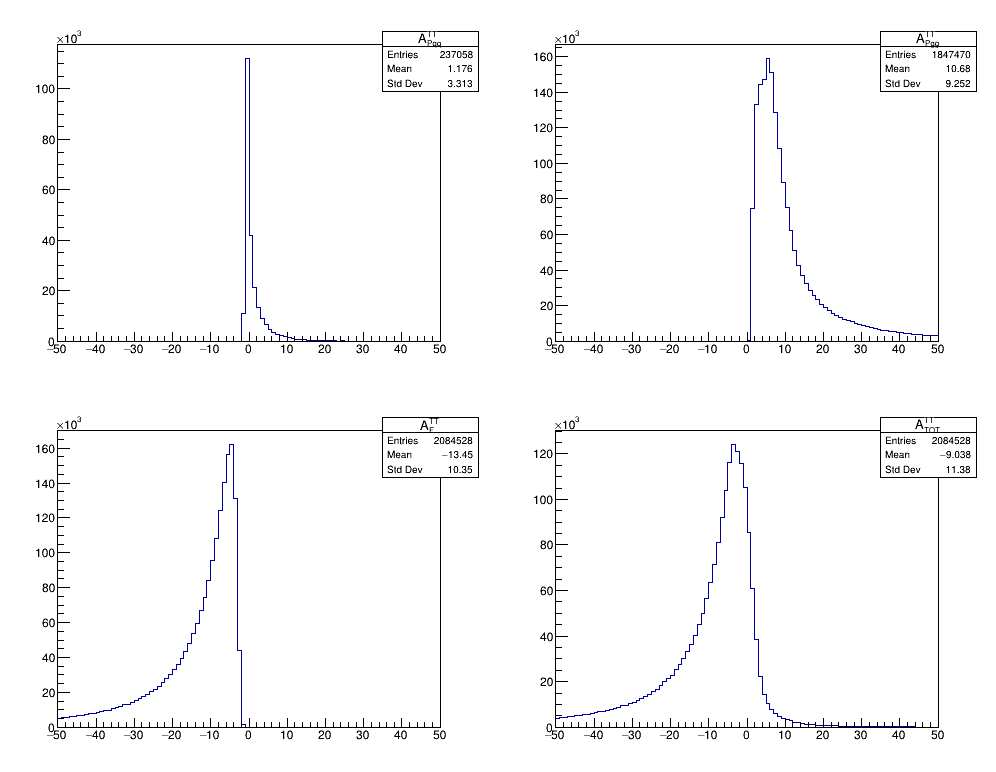
\includegraphics[scale=0.2]{amunuTT.png}
        \end{center}
        \caption{Distribution pour $ A^\mathrm{TT} $}
    \end{figure}
\end{minipage}%
\begin{minipage}{0.5\textwidth}
    \begin{figure}[H]
        \begin{center}
         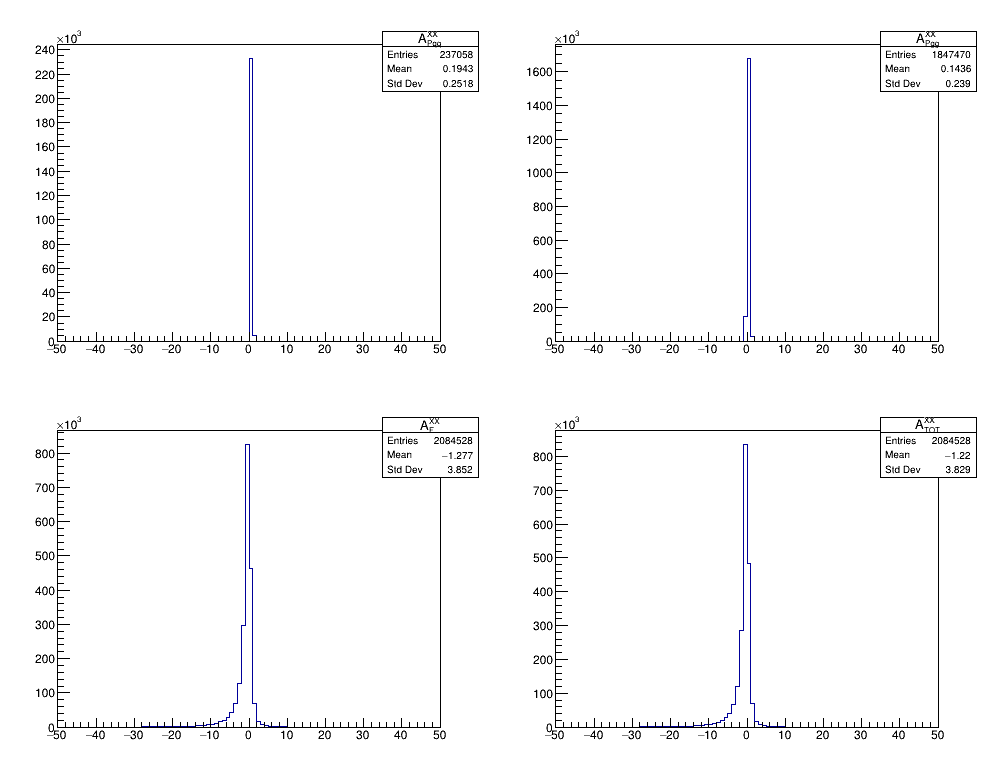
\includegraphics[scale=0.2]{amunuXX.png}
        \end{center}
        \caption{Distribution pour $ A^\mathrm{XX} $}
    \end{figure}
\end{minipage}%

\begin{minipage}{0.5\textwidth}
    \begin{figure}[H]
        \begin{center}
         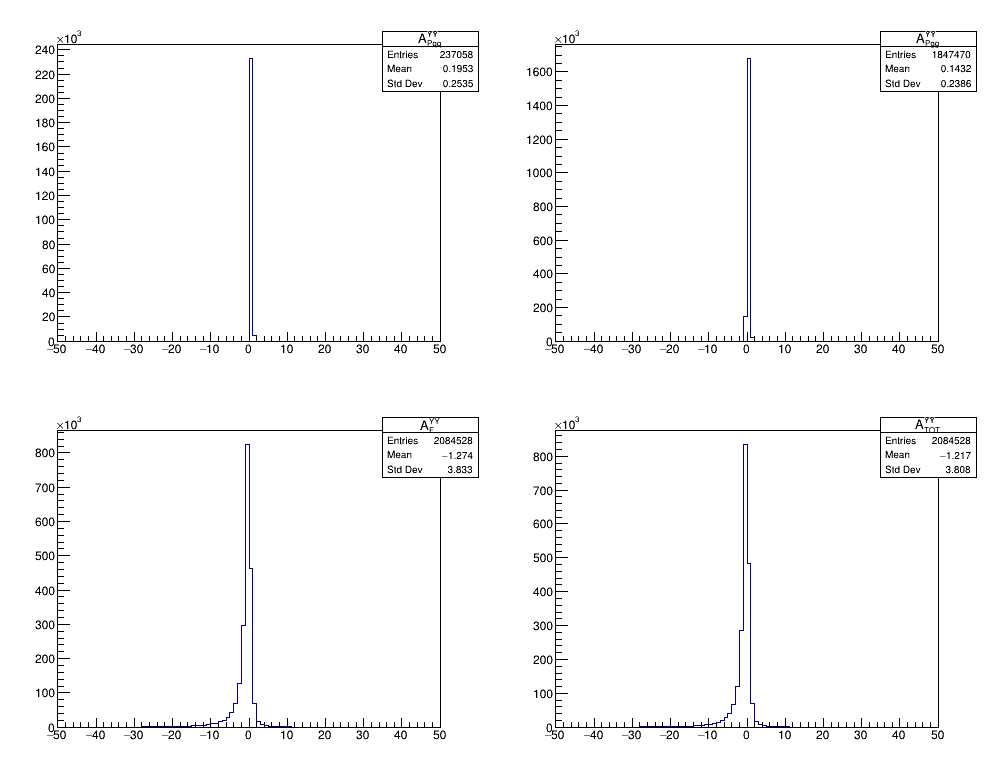
\includegraphics[scale=0.2]{amunuYY.png}
        \end{center}
                \caption{Distribution pour $ A^\mathrm{YY} $}
    \end{figure}
\end{minipage}%
\begin{minipage}{0.5\textwidth}
    \begin{figure}[H]
        \begin{center}
         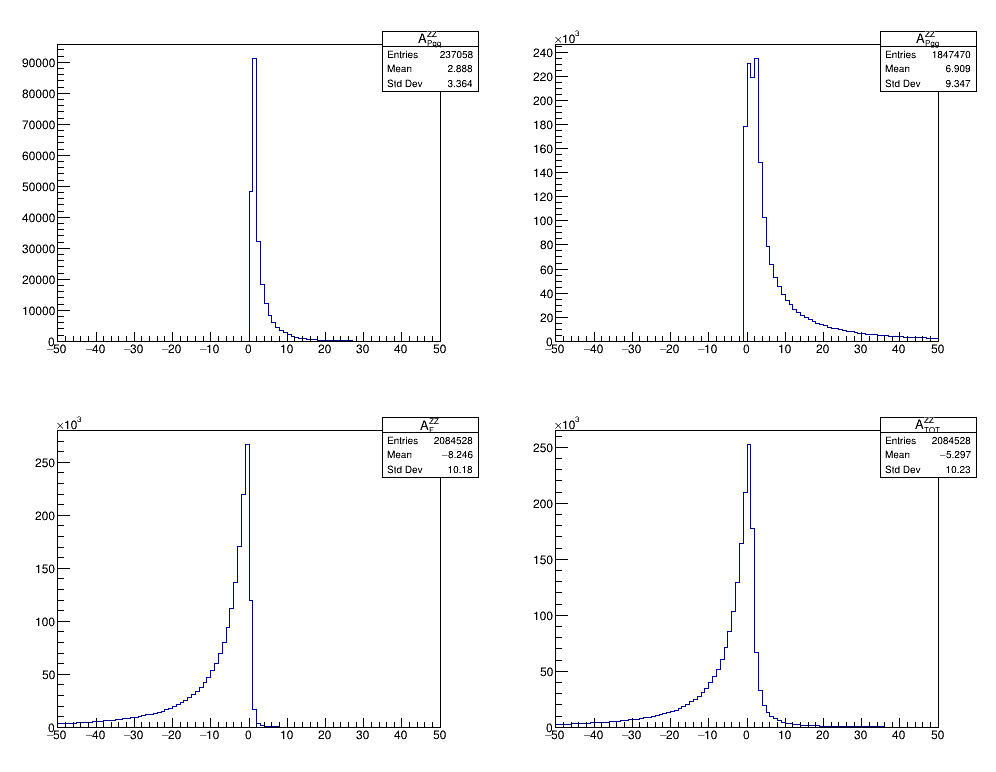
\includegraphics[scale=0.2]{amunuZZ.png}
        \end{center}
        \caption{Distribution pour $ A^\mathrm{ZZ} $}
    \end{figure}
\end{minipage}%


\begin{minipage}{0.5\textwidth}
    \begin{figure}[H]
        \begin{center}
         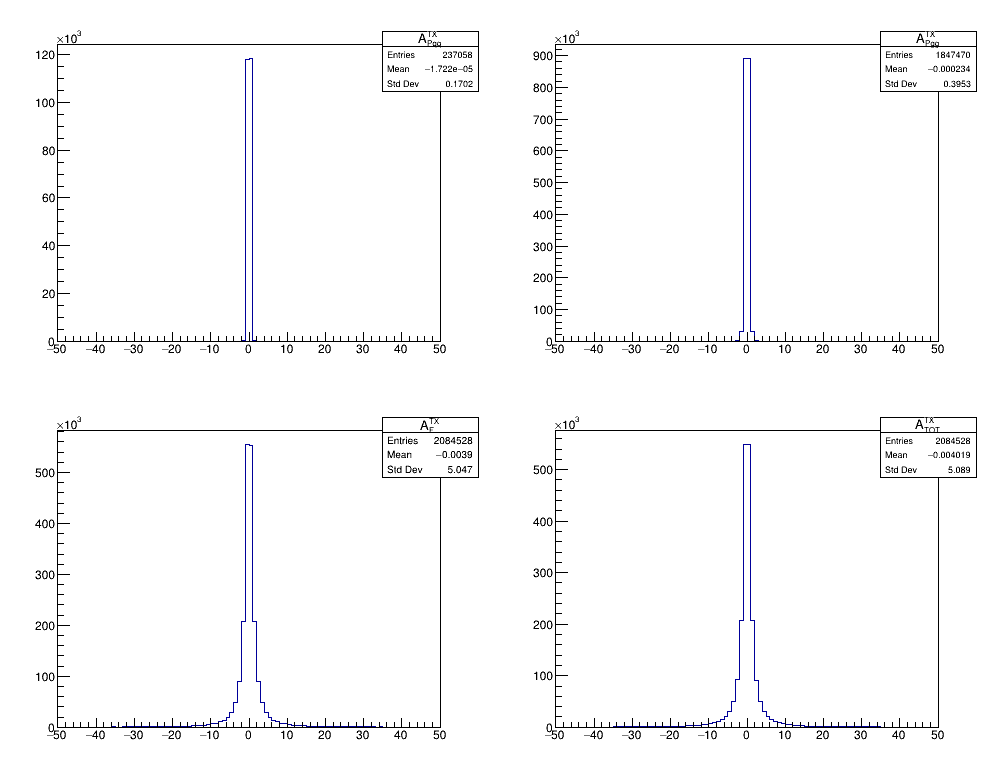
\includegraphics[scale=0.2]{amunuTX.png}
        \end{center}
        \caption{Distribution pour $ A^\mathrm{TX}$ et $ A^\mathrm{XT}$}
    \end{figure}
\end{minipage}%
\begin{minipage}{0.5\textwidth}
    \begin{figure}[H]
        \begin{center}
         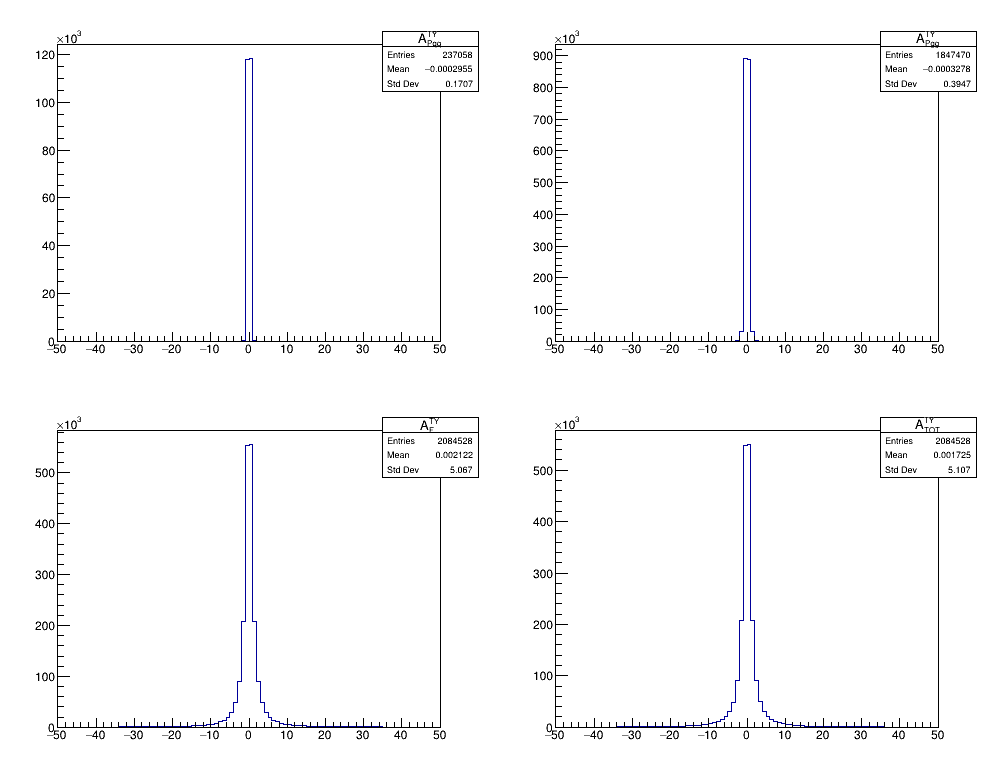
\includegraphics[scale=0.2]{amunuTY.png}
        \end{center}
           \caption{Distribution pour $ A^\mathrm{TY}$ et $ A^\mathrm{YT}$}     
    \end{figure}
\end{minipage}%

\begin{minipage}{0.5\textwidth}
    \begin{figure}[H]
        \begin{center}
         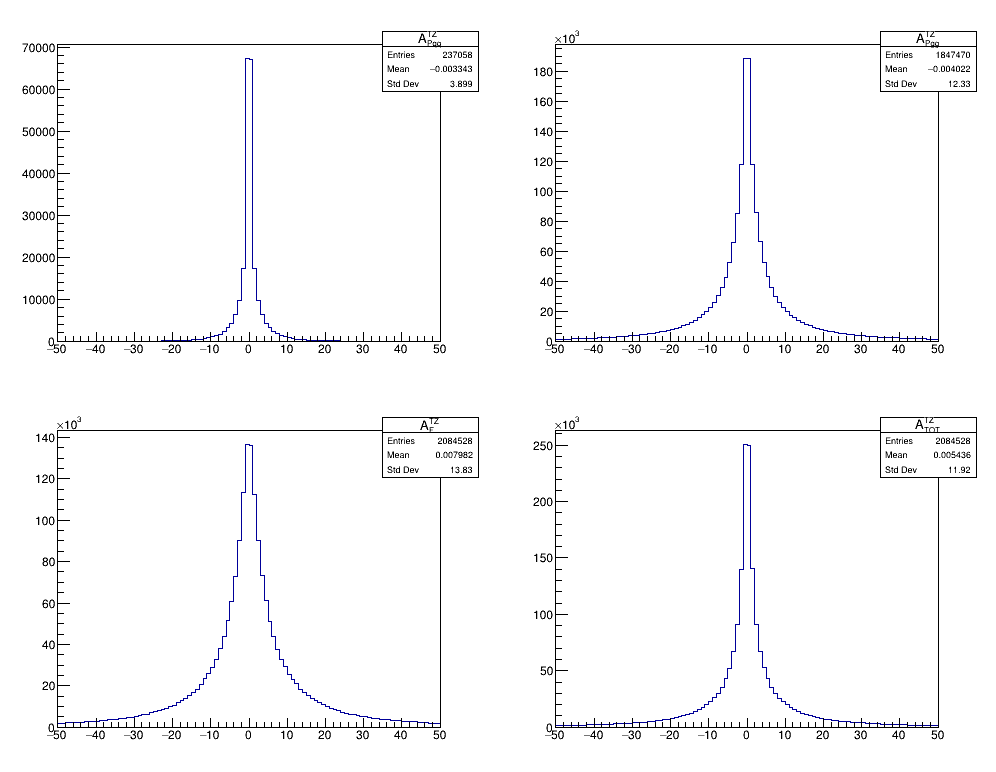
\includegraphics[scale=0.2]{amunuTZ.png}
        \end{center}
            \caption{Distribution pour $ A^\mathrm{TZ}$ et $ A^\mathrm{ZT}$}    
    \end{figure}
\end{minipage}%
\begin{minipage}{0.5\textwidth}
    \begin{figure}[H]
        \begin{center}
         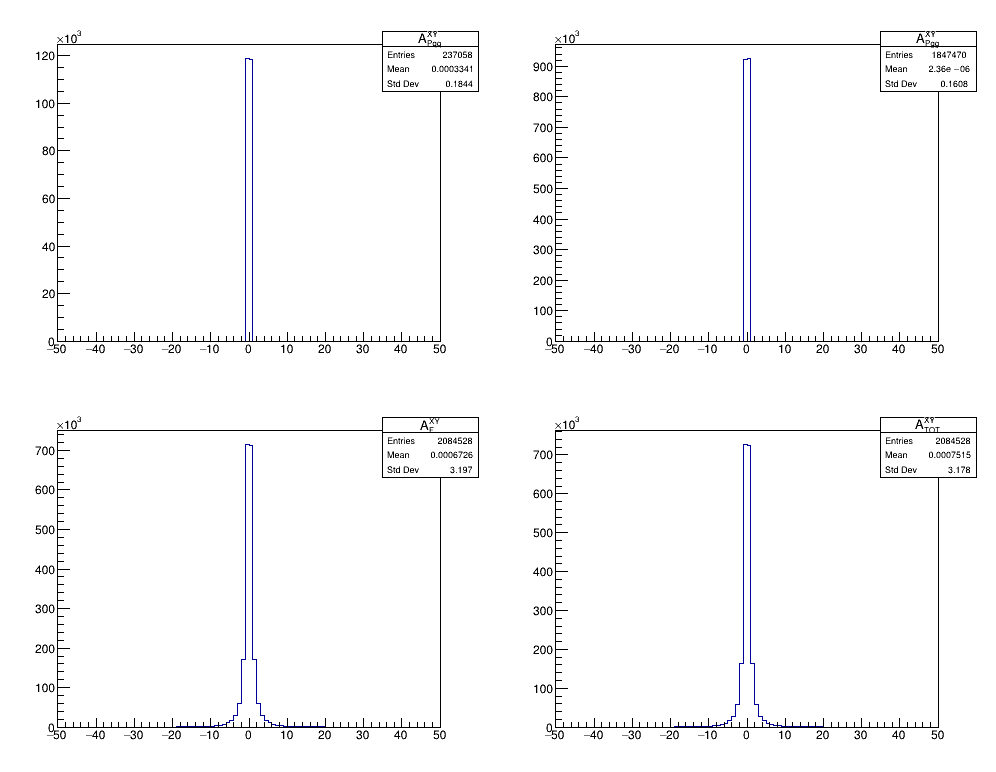
\includegraphics[scale=0.2]{amunuXY.png}
        \end{center}
        \caption{Distribution pour $ A^\mathrm{XY}$ et $ A^\mathrm{YX}$}
    \end{figure}
\end{minipage}%

\begin{minipage}{0.5\textwidth}
    \begin{figure}[H]
        \begin{center}
         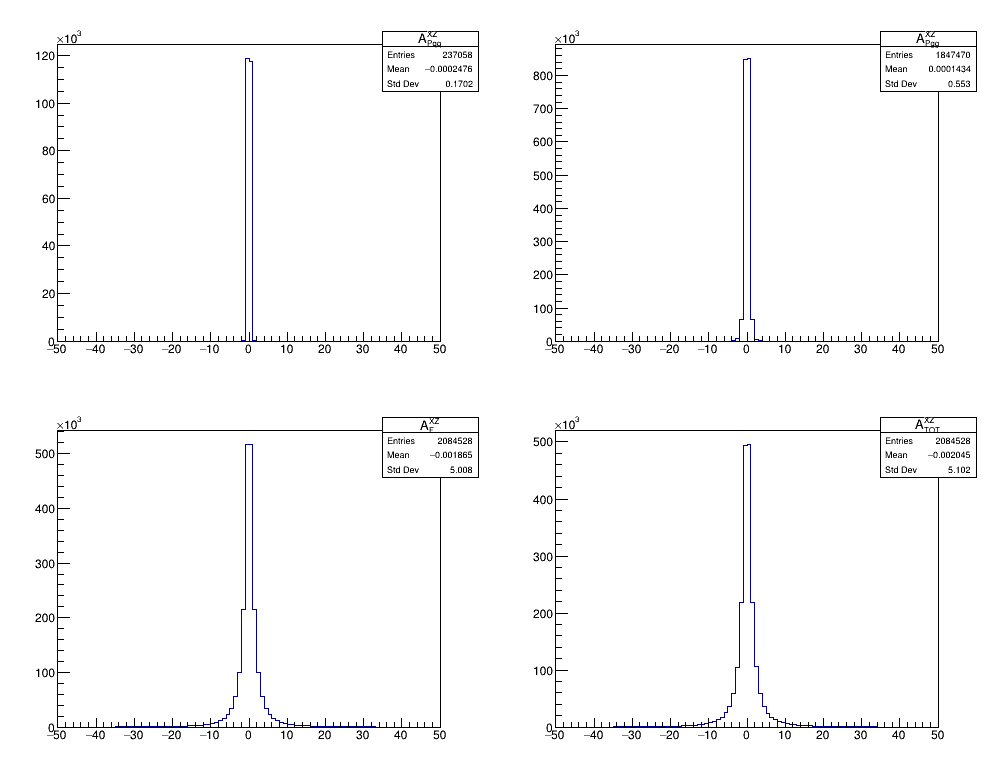
\includegraphics[scale=0.2]{amunuXZ.png}
        \end{center}
        \caption{Distribution pour $ A^\mathrm{XZ}$ et $ A^\mathrm{ZX}$}
    \end{figure}
\end{minipage}%
\begin{minipage}{0.5\textwidth}
    \begin{figure}[H]
        \begin{center}
         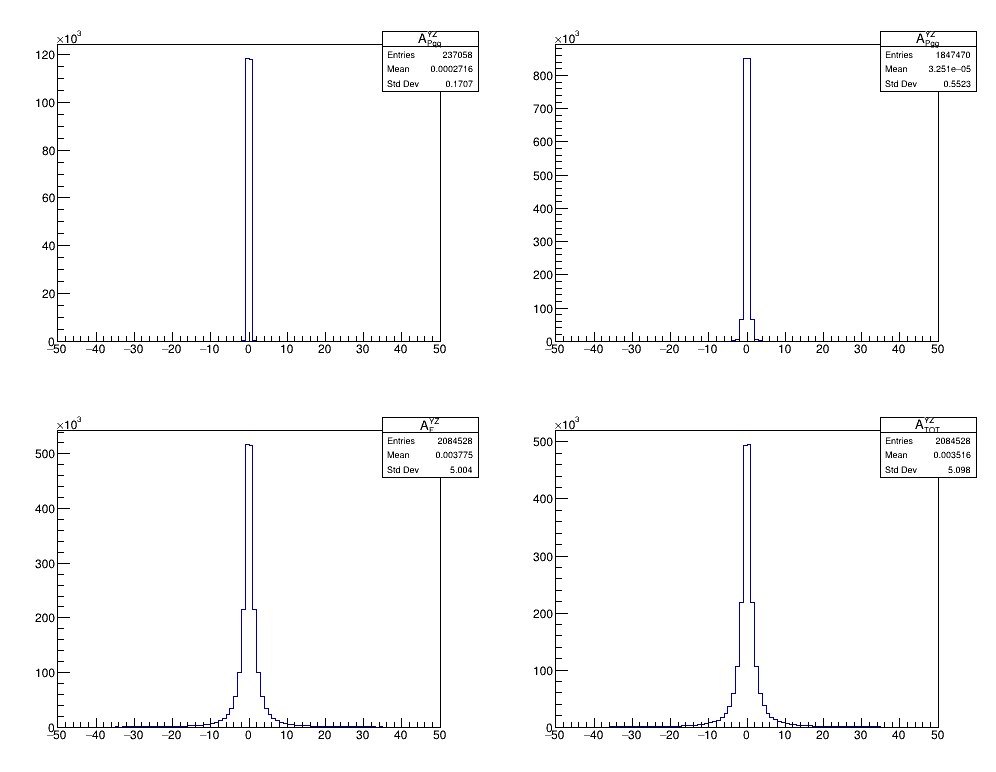
\includegraphics[scale=0.2]{amunuYZ.png}
        \end{center}
        \caption{Distribution pour $ A^\mathrm{YZ}$ et $ A^\mathrm{ZY}$}
    \end{figure}
\end{minipage}%


    \section{Les fonctions $f(t)$}\label{B:f}

Dans cette section sont développées les formes des fonctions de modulation $f(t)$ pour les autres couples non-nuls de coefficients $c_{\mu\nu}$.

        \subsection{$c_\mathrm{XY} = c_\mathrm{YX}$}
            Considérons que seuls $c_\mathrm{XY} = c_\mathrm{YX}$ sont non nuls. On a :
            \begin{align*}
                \frac{f_\mathrm{SME}^{\mathrm{(XY)}} (t)}{2 c_\mathrm{XY}} & = \left( \left(R_X^X R_X^Y + R_Y^X R_Y^Y \right) \langle A^\mathrm{XX} \rangle  +  R_Z^X R_Z^Y \langle A^\mathrm{ZZ} \rangle   \right)
                \\ & =  \left( (- c_t s_\lambda s_\theta + s_t c_\theta)(- s_t s_\lambda s_\theta - c_t c_\theta) + c_t s_t c_\lambda^2 \right) \langle A^\mathrm{XX} \rangle
                \\ & \qquad + (- c_t s_\lambda c_\theta - s_t s_\theta)(- s_t s_\lambda c_\theta - c_t s_\theta) \langle A^\mathrm{ZZ} \rangle
                \\ & = \underbrace{\left( \left( s_\lambda^2 s_\theta^2 + c_\lambda^2 \right) \langle A^\mathrm{XX} \rangle +s_\lambda^2 c_\theta^2 \langle A^\mathrm{ZZ} \rangle \right)}_{a_1} c_t s_t - \underbrace{\left( c_\theta^2 \langle A^\mathrm{XX} \rangle + s_\theta^2 \langle A^\mathrm{ZZ} \rangle  \right)}_{a_2} c_t s_t
                \\ & \qquad - \underbrace{s_\lambda c_\theta s_\theta \left(\langle A^\mathrm{ZZ} \rangle  - \langle A^\mathrm{XX} \rangle \right) }_{a_3}  \left( c_t^2 - s_t^2 \right)
                \\ & = \frac{a_1}{2} \sin(2\Omega t) - \frac{a_2}{2} \sin(2 \Omega t) - a_3 \cos(2\Omega t)
            \end{align*}
            \begin{equation}
                \boxed{f_\mathrm{SME}^{\mathrm{(XY)}} (t) = 2 c_\mathrm{XY} \left( \left( \frac{a_1 - a_2}{2} \right)  \sin(2 \Omega t) - a_3 \cos(2 \Omega t)  \right)}
            \end{equation}
        \subsection{$c_\mathrm{XZ} = c_{ZX}$}
            Considérons que seuls $c_\mathrm{XZ} = c_{ZX}$ sont non nuls. On a :
            \begin{align*}
                \frac{f_\mathrm{SME}^{\mathrm{(XZ)}} (t)}{2 c_\mathrm{XZ}} & = \left( \left(R_X^X R_X^Z + R_Y^X R_Y^Z \right) \langle A^\mathrm{XX} \rangle  +  R_Z^X R_Z^Z \langle A^\mathrm{ZZ} \rangle   \right)
                \\ & = \left( (- c_t s_\lambda s_\theta + s_t c_\theta)(-c_\lambda s_\theta) + (c_t c_\lambda)(-s_\lambda) \right) \langle A^\mathrm{XX} \rangle + (c_t s_\lambda c_\theta + s_t 	s_\theta)(c_\lambda\ c_\theta ) \langle A^\mathrm{ZZ} \rangle
                \\ & = -c_t \underbrace{c_\lambda s_\lambda \left( \left(1 - s_\theta^2 \right) \langle A^\mathrm{XX} \rangle - c_\theta^2 \langle A^\mathrm{ZZ} \rangle  \right) }_{c_\lambda s_\lambda c_\theta^2 \left( \langle A^\mathrm{ZZ} \rangle  - \langle A^\mathrm{XX} \rangle  \right) = a_4} + s_t \underbrace{s_\theta c_\lambda c_\theta \left( \langle A^\mathrm{ZZ} \rangle - \langle A^\mathrm{XX}  \rangle \right)}_{a_5}
            \end{align*}
            \begin{equation}
                \boxed{f_\mathrm{SME}^{\mathrm{(XZ)}} (t)  = 2 c_\mathrm{XZ} \left(a_4 \cos(\Omega t) + a_5 \sin(\Omega t) \right)}
            \end{equation}
        \subsection{$c_\mathrm{YZ} = c_\mathrm{ZY}$}
            Considérons que seuls $c_\mathrm{YZ} = c_\mathrm{ZY}$ sont non nuls. On a :
            \begin{align*}
                \frac{f_\mathrm{SME}^{\mathrm{(YZ)}} (t)}{2 c_\mathrm{YZ}} & = \left( \left(R_X^Y R_X^Z + R_Y^Y R_Y^Z \right) \langle A^\mathrm{XX} \rangle  +  R_Z^Y R_Z^Z \langle A^\mathrm{ZZ} \rangle   \right)
                \\ & = \left( ( - s_t s_\lambda s_\theta - c_t c_\theta )( -c_\lambda s_\theta) + ( s_t c_\lambda)( -s_\lambda) \right) \langle A^\mathrm{XX} \rangle + ( s_t s_\lambda c_\theta - c_t s_\theta )(c_\lambda c_\theta ) \langle A^\mathrm{ZZ} \rangle
                \\ & = -c_t \underbrace{s_\theta c_\lambda c_\theta \left( \langle A^\mathrm{ZZ} \rangle - \langle A^\mathrm{XX}  \rangle \right)}_{a_5} + s_t \underbrace{c_\lambda s_\lambda \left( \left(1 - s_\theta^2 \right) \langle A^\mathrm{XX} \rangle - c_\theta^2 \langle A^\mathrm{ZZ} \rangle  \right) }_{a_4}
            \end{align*}
            \begin{equation}
                \boxed{f_\mathrm{SME}^{\mathrm{(YZ)}} (t)  = 2 c_\mathrm{YZ} \left(a_4 \sin(\Omega t) - a_5 \cos(\Omega t) \right)}
            \end{equation}


    \subsection{Les cas $c_{Ti}$ avec $i=X,Y,Z$}
        Considérons que seuls $c_{TX} = c_{XT}$ sont non nuls. On a :
        \begin{align*}
            \frac{f_\text{SME}^{(TX)}(t)}{2c_{TX}} &= R^X_X \langle A^{TX} \rangle +  R^X_Y \langle A^{TY} \rangle +  R^X_Z \langle A^{TZ} \rangle
            \\ &= \left( -c_t s_\lambda s_\theta + s_t c_\theta \right) \langle A^{TX} \rangle + \left( c_t c_\lambda \right) \langle A^{TY} \rangle + \left( c_t s_\lambda c_\theta + s_t s_\theta  \right)\langle A^{TZ} \rangle
            \\ &= \underbrace{\left( -s_\lambda s_\theta \langle A^{TX} \rangle + c_\lambda \langle A^{TY} \rangle + s_\lambda c_\theta \langle A^{TZ} \rangle \right)}_{b_1} c_t + \underbrace{c_\theta  \langle A^{TX} \rangle  + s_\theta \langle A^{TZ} \rangle}_{b_2} s_t
            \\ &= b_1 \cos(\Omega t) + b_2 \sin(\Omega t)
        \end{align*}
        \begin{equation}
            \boxed{f_\text{SME}^{(TX)}(t) = 2c_{TX} \left( b_1 \cos(\Omega t) + b_2 \sin(\Omega t) \right)}
        \end{equation}
        Considérons que seuls $c_{TY} = c_{YT}$ sont non nuls. On a :
        \begin{align*}
            \frac{f_\text{SME}^{(TY)}(t)}{2c_{TY}} &= R^Y_X \langle A^{TX} \rangle +  R^Y_Y \langle A^{TY} \rangle +  R^Y_Z \langle A^{TZ} \rangle
            \\ &= \left( -s_t s_\lambda s_\theta - c_t c_\theta \right) \langle A^{TX} \rangle + \left( s_t c_\lambda \right) \langle A^{TY} \rangle + \left( s_t s_\lambda c_\theta - c_t s_\theta  \right)\langle A^{TZ} \rangle
            \\ &= \underbrace{\left( -s_\lambda s_\theta \langle A^{TX} \rangle + c_\lambda \langle A^{TY} \rangle + s_\lambda c_\theta \langle A^{TZ} \rangle \right)}_{b_1} s_t - \underbrace{ \left( c_\theta  \langle A^{TX} \rangle  + s_\theta \langle A^{TZ} \rangle \right)}_{b_2} c_t
            \\ &= b_1 \sin(\Omega t) - b_2 \cos(\Omega t)
        \end{align*}
        \begin{equation}
            \boxed{f_\text{SME}^{(TY)}(t) = 2c_{TY} \left( b_1 \sin(\Omega t) - b_2 \cos(\Omega t) \right)}
        \end{equation}

        
        \section{Tracés des coefficients de Wilson}\label{B:wilson}
Dans cette section sont présentées les modulations de tout les couples non-nuls d'un coefficient donné fixé à 0,1. Ce, dans le scenario du Run II du LHC à $13\,\mathrm{TeV}$ avec une luminosité $\mathcal{L} = 150\,\mathrm{fb}^{-1}$.
        \subsection{$c_{R\mu\nu} $}
            \begin{figure}[H]
                \begin{center}
                    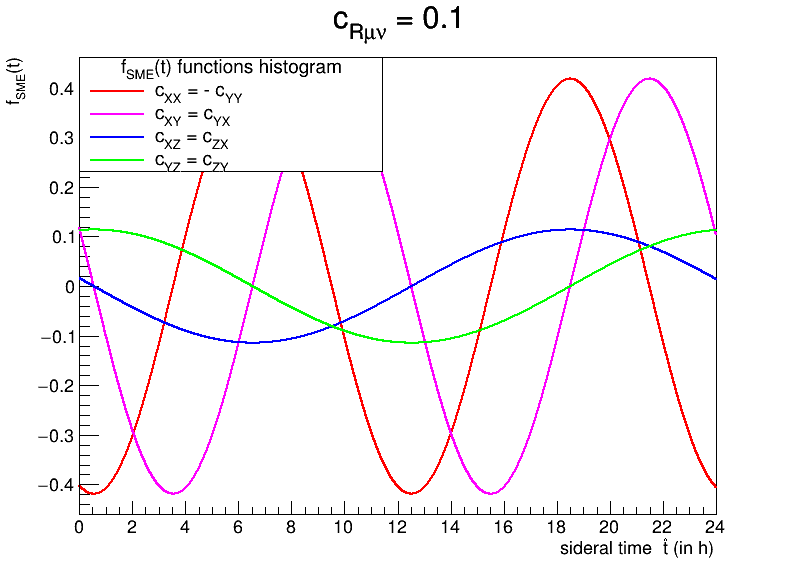
\includegraphics[scale=0.4]{fComparaisonR.png}
                    \caption{LHC 13TeV}
                \end{center}
            \end{figure}
            
        \subsection{$c_{\mu\nu} $}
            \begin{figure}[H]
                \begin{center}
                    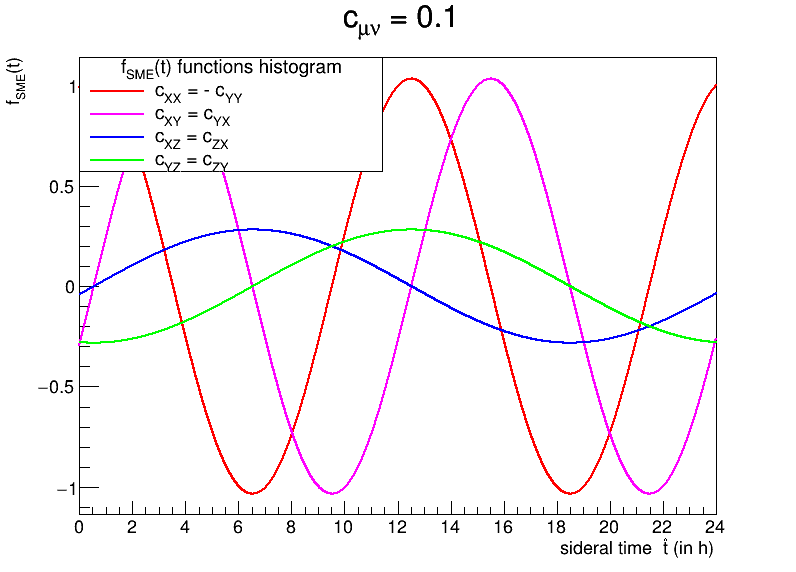
\includegraphics[scale=0.4]{fComparaisonC.png}
                    \caption{LHC 13TeV}
                \end{center}
            \end{figure}

        \subsection{$d_{\mu\nu} $}
            \begin{figure}[H]
                \begin{center}
                    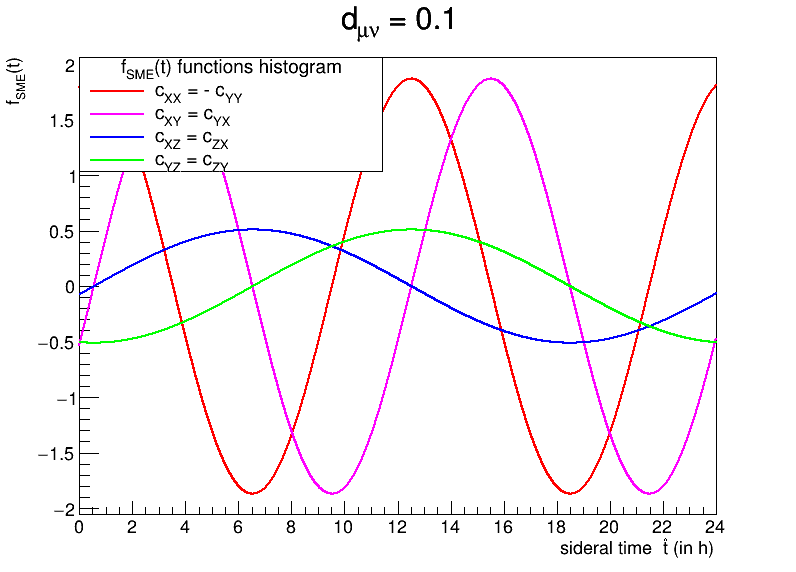
\includegraphics[scale=0.4]{fComparaisonD.png}
                    \caption{LHC 13TeV}
                \end{center}
            \end{figure}

\section{Moyenne d'éléments de matrice $\langle A_{\mu\nu} \rangle$}\label{B:averageamunu}

Dans cette section est présentée sous forme d'histogramme, la différence entre l'évaluation de la modulation pour un couple de coefficients donné, en bins de temps, avec utilisation d'une matrice  $ A^{\mu\nu} $ moyenne et sans. Ceci montre la pertinence de l'utilisation des matrices moyennes. En effet, que l'on bin une fonction composée d'une matrice $A_{\mu\nu}$ par évènement ou que l'on bin la fonction analytique générée à partir de la moyenne  $\langle A_{\mu\nu} \rangle$ sur tous les évènements, on obtient un résultat similaire.

        \begin{figure}[H]
            \begin{center}
                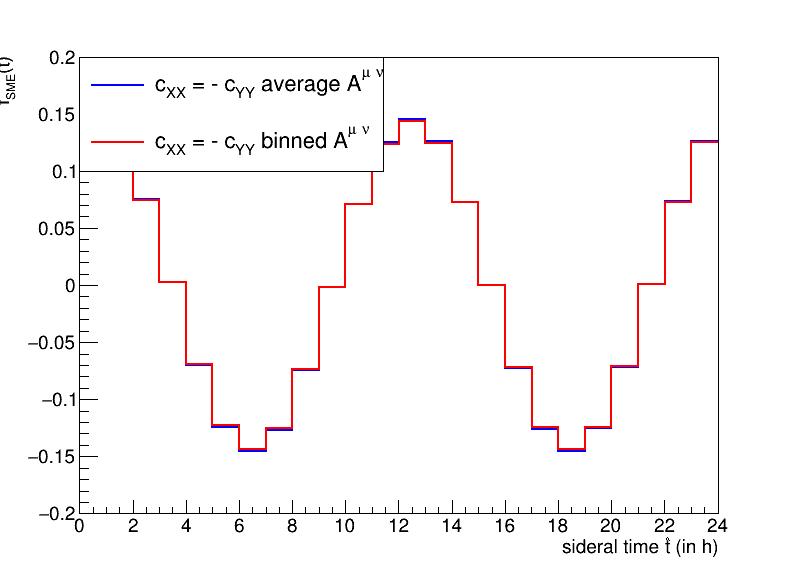
\includegraphics[scale=0.4]{biais24fComparaison.png}
                \caption{Moyenne de la composante cinétique en 24 bins}
            \end{center}
            \begin{center}
                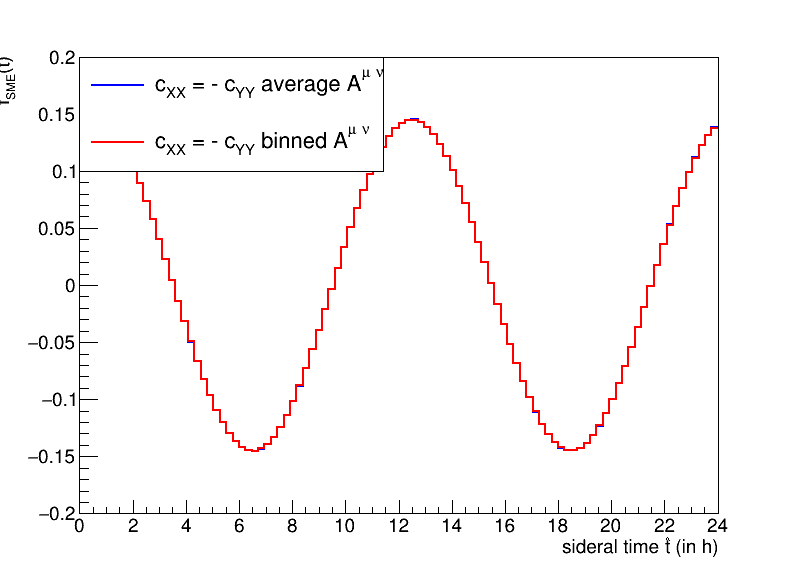
\includegraphics[scale=0.4]{biais100fComparaison.png}
                \caption{Moyenne de la composante cinétique en 100 bins}
            \end{center}
        \end{figure}

\section{Maximum de modulation fonction de la latitude et de l'azimut}\label{B:max}

Cette section présente les formes des équations de maximum de modulation en fonction de la latitude et de l'azimut.

\subsection{$c_\mathrm{XX} = -c_\mathrm{YY}$}
\begin{align*}
    f^\mathrm{(XX)'}(t_\mathrm{max}) &= 2 c_\mathrm{XX} \left( -2\Omega \left( \frac{a_1 - a_2}{2} \right) \sin(2\Omega t_\mathrm{max} ) + 2\Omega a_3 \cos(2\Omega t_\mathrm{max})\right) \\
    &=  -\left( \frac{a_1 - a_2}{2} \right) \sin(2\Omega t_\mathrm{max} ) + a_3 \cos(2\Omega t_\mathrm{max})  \\ 
     &= \frac{a_1 - a_2}{2a_3} -  \cot(2\Omega t_\mathrm{max}) \\
     &= 0 
\end{align*}
Le maximum d'oscillation est obtenu à :
\begin{equation*}\boxed{
    t_\mathrm{max} = \frac{1}{2\Omega} \cot^{-1}\left( \frac{a_1 - a_2}{2a_3}  \right)}
\end{equation*}

\subsection{$c_\mathrm{XY} = c_\mathrm{YX}$}
\begin{align*}
    f^\mathrm{\mathrm{(XY)}'}(t_\mathrm{max}) &= 2 c_\mathrm{XY} \left( 2\Omega \left( \frac{a_1 - a_2}{2} \right) \cos(2\Omega t_\mathrm{max} ) + 2\Omega a_3 \sin(2\Omega t_\mathrm{max})\right) \\
    &=  \left( \frac{a_1 - a_2}{2} \right) \cos(2\Omega t_\mathrm{max} ) + a_3 \sin(2\Omega t_\mathrm{max})  \\ 
     &= \frac{a_1 - a_2}{2a_3} +  \tan(2\Omega t_\mathrm{max}) \\
     &= 0 
\end{align*}
Le maximum d'oscillation est obtenu à :
\begin{equation*}\boxed{
    t_\mathrm{max} = \frac{1}{2\Omega} \arctan\left( \frac{a_2 - a_1}{2a_3}  \right)}
\end{equation*}

\subsection{$c_\mathrm{XZ} = c_{ZX}$}
\begin{align*}
    f^\mathrm{\mathrm{(XZ)}'}(t_\mathrm{max}) &= 2 c_\mathrm{XZ} \left( -\Omega a_4 \sin(\Omega t_\mathrm{max} ) + \Omega a_5 \cos(\Omega t_\mathrm{max})\right) \\
     &= -\frac{a_5}{a_4} +  \tan(\Omega t_\mathrm{max}) \\
     &= 0 
\end{align*}
Le maximum d'oscillation est obtenu à :
\begin{equation*}\boxed{
    t_\mathrm{max} = \frac{1}{\Omega} \arctan\left( \frac{a_5}{a_4}  \right)}
\end{equation*}

\subsection{$c_\mathrm{YZ} = c_\mathrm{YX}$}
\begin{align*}
    f^\mathrm{\mathrm{(XZ)}'}(t_\mathrm{max}) &= 2 c_\mathrm{XZ} \left( \Omega a_4 \cos(\Omega t_\mathrm{max} ) + \Omega a_5 \sin(\Omega t_\mathrm{max})\right) \\
     &= \frac{a_4}{a_5} +  \tan(\Omega t_\mathrm{max}) \\
     &= 0 
\end{align*}
Le maximum d'oscillation est obtenu à :
\begin{equation*}\boxed{
    t_\mathrm{max} = \frac{1}{\Omega} \arctan\left(- \frac{a_4}{a_5}  \right)}
\end{equation*}

\begin{figure}[H]
    \begin{center}
        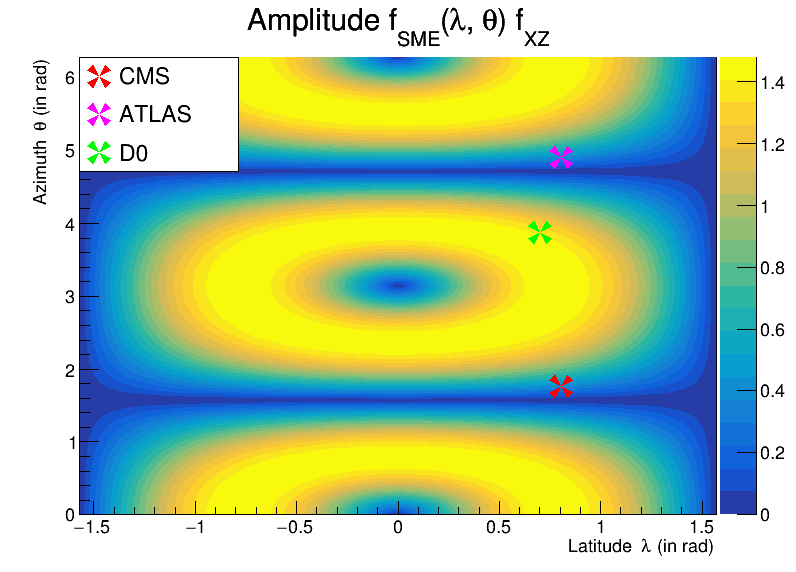
\includegraphics[scale=0.4]{XZ.png}
        \caption{Amplitude de $f(\lambda, \theta)$ en fonction de la latitude et de l'azimut pour $c_\mathrm{XZ}= c_\mathrm{ZX}$ dans un scénario à $13\,\mathrm{TeV}$ avec les orientations de détecteurs CMS, ATLAS et D$\emptyset$.}
        \label{B:orientation}
    \end{center}
\end{figure}



\end{fmffile}
